
%(BEGIN_QUESTION)
% Copyright 2006, Tony R. Kuphaldt, released under the Creative Commons Attribution License (v 1.0)
% This means you may do almost anything with this work of mine, so long as you give me proper credit

Write equations expressing the total voltage sensed by the indicating instrument, as functions of the voltages shown in the diagrams.  Assume that all junctions form the same thermocouple type (e.g. all type J, all type K, etc.):

$$\includegraphics[width=15.5cm]{i00399x01.eps}$$

\underbar{file i00399}
%(END_QUESTION)





%(BEGIN_ANSWER)

\noindent
{\bf Series:}

$$V_{meter} = (V_1 + V_3 + V_5) - (V_2 + V_4 + V_{ref})$$

\vskip 10pt

\noindent
{\bf Parallel:}

$$V_{meter} = {{V_1 + V_2 + V_3} \over 3} - V_{ref}$$

\vskip 10pt

Follow-up question: explain why {\it swamping resistors} are often added to paralleled thermocouples to improve the accuracy of their temperature averaging:

$$\includegraphics[width=15.5cm]{i00399x02.eps}$$

%(END_ANSWER)





%(BEGIN_NOTES)

The swamping resistors ``swamp out'' differences in thermocouple lead resistance.  This is quite important when the thermocouple cables differ significantly in length.

%INDEX% Measurement, temperature: series and parallel thermocouples

%(END_NOTES)


